\chapter{Librerías de programación orientadas al web scraping}
\label{cha:librerias de programacion orientadas al web scraping}

\section{Búsqueda de librerías destinadas al web scraping}
\label{sec:busqueda de librerias destinadas al web scraping}

Como se especificó en la sección \ref{sec:objetivo y limitaciones} este trabajo se limitará a realizar
una comparativa de los programas software de minado web más frecuentes. Esta comparativa se efectúa con el
fin de conocer cuál o cuáles de estos programas o paquetes software son los más rentables para este propósito.

¿Como saber que paquetes software destinados al minado web son los más comunes? Durante todo este capítulo
se procederá a la búsqueda, selección e introducción de programas software empleados para el web scraping. 
Cabe destacar que Python y R serán los lenguajes de programación con los que se trabajará tanto para el 
desarrollo de la herramienta de comparación, como para el proceso de extracción de datos.

El primer paso consiste en buscar todos los elementos posibles que conforman la población de paquetes
software del mercado, ya sean de Python o R. La búsqueda de estos paquetes se ha realizado a través de las 
distintas fuentes de información mostradas a continuación:

\begin{enumerate}
  \item GitHub \cite{github}. Gran parte de los desarrolladores de estos programas, publican su trabajo en
  estos repositorios de código abierto.
  \item CRAN \cite{cran}. The Comprehensive R Archive Network es una red de servidores ftp y web que
  almacena versiones idénticas de código y documentación para R.
  \item PyPi \cite{pypi}. Python Package Index es un repositorio de software para Python, útil para la
  búsqueda de paquetes de un determinado propósito.
\end{enumerate}

\section{Librerías de Python encontradas durante el proceso de búsqueda}
\label{sec:librerias de python encontradas durante el proceso de busqueda}

A continuación, se hará una breve sinopsis de las librerías encontradas en Python. Esta introducción tiene
como objetivo conocer el funcionamiento de los paquetes, cuáles son sus funciones y como es el proceso de
extracción.

Es posible que algunos de los paquetes hayan sido desarrollados tanto en R como en Python. En ese caso, por 
un lado, la introducción se realzará de forma conjunta, sin embargo, será interesante ver el código del 
mismo en ambos casos y como se comportan estos ante los distintos test de evaluación.

Antes de comenzar con la sinopsis de paquetes, es conveniente revisar el apéndice \ref{cha:analizadores
empleados en el web scraping}, donde se realiza una breve introducción de aquellos analizadores empleados
en los mismos. Los 'emparejamientos' entre biblioteca-analizador se recogen en la tabla 
\ref{tab:emparejamientos biblioteca-analizador} a modo de resumen.

\begin{table}[h]
  \begin{center}
  \begin{tabular}{| c | c | c | c | c | c | c | c |} \hline 
    \textbf{htmltext} & \textbf{inscriptis} & \textbf{dragnet} & \textbf{boilerpy} & \textbf{newspaper} & \textbf{newsplease} & \textbf{justext} & \textbf{goose3} \\ \hline
    lxml etree & lxml html & lxml etree & html parser & lxml etree & lxml etree & lxml html & lxml html \\ \hline
  \end{tabular}

  \hfill \break

  \begin{tabular}{| c | c | c | c | c |} \hline 
    \textbf{readability} & \textbf{trafilatura} & \textbf{beautifulsoup} & \textbf{libextract} & \textbf{html2text}  \\ \hline
    lxml html \& etree & lxml html \& etree & lxml etree \& html5lib \& html parser & lxml html & html parser \\ \hline
  \end{tabular}

  \caption{Emparejamientos biblioteca-analizador}
  \label{tab:emparejamientos biblioteca-analizador}
  \end{center}
\end{table}

Ya sea porque determinadas bibliotecas permiten al desarrollador seleccionar entre varios tipos de 
analizadores, o bien porque múltiples de ellos son necesarios para el correcto funcionamiento de la 
extracción, muchas de estas bibliotecas hacen uso de más de un analizador en su código.

\subsection{Inscriptis}
\label{subsec:inscriptis}

\emph{Inscriptis} \cite{inscriptis} además de ser una biblioteca de conversión de HTML a texto basada en
Python, también tiene soporte como línea de comandos o como servicio web para tablas anidadas. A pesar de
sus múltiples funcionalidades, a lo largo de esta sección nos centraremos en inscriptis como biblioteca
de programación.

\subsubsection{Estructura de la solución}
\label{subsubsec:estructura de la solucion}

A diferencia de otros algoritmos de extracción, Inscriptis no solo tiene en cuenta la calidad del texto
extraído, la estructura del mismo también es muy importante. Esto provoca que el resultado obtenido se
acerque más a un posible resultado aplicando el método tradicional a través de cualquier navegador web.

Veamos una pequeña comparación entre la extracción de texto de Beautiful Soup \ref{subsec:beautiful soup}, 
con la extracción de texto de Inscriptis, donde se tiene un fragmento HTML como el siguiente como objeto 
de prueba.

\begin{Schunk}
  \begin{Soutput}
      <li>first</li>
      <li>second</li>
  \end{Soutput}
\end{Schunk}

Empleamos en primer lugar el metodo \emph{get\_text()} propio de Beautiful Soup sobre el fragmento HTML
anterior. Veamos cuál es el resultado.

\begin{Schunk}
  \begin{Soutput}
    # firstsecond
  \end{Soutput}
\end{Schunk}

Se puede observar que el formato obtenido no es el adecuado, puesto que no se ha respetado la estructura
del documento base. Sin embargo, si aplicamos Inscriptis sobre el mismo fragmento HTML, la salida obtenida
sería la siguiente:

\begin{Schunk}
  \begin{Soutput}
    # first
    # second
  \end{Soutput}
\end{Schunk}

El algoritmo no solo admite construcciones tan simples como la anterior, tambien es posible analizar 
construcciones mucho más complejas, como las tablas anidadas, y subconjuntos de atributos HTML o CSS donde 
es esencial una conversión precisa de HTML a texto.

\subsubsection{Reglas de anotación}
\label{subsubsec:reglas de anotacion}

La técnica que emplea Inscriptis se conoce como reglas de anotación, es decir, mapeos que permiten realizar 
anotaciones sobre el texto extraído. Estas anotaciones se basan en la información estructural y semántica 
codificada en las etiquetas y atributos HTML utilizados para controlar la estructura y diseño del documento 
original. Con el fin de asignar etiquetas y/o atributos HTML a las anotaciones, se emplea lo que se conoce 
como perfil de anotaciones, algo parecido a un diccionario. 


\begin{table}[h]
  \begin{center}
  \begin{tabular}{| c | c |} \hline 
    h1 & ['heading', 'h1'] \\ \hline
    h2 & ['heading', 'h2'] \\ \hline
    b & ['emphasis'] \\ \hline
    div\#class=toc & ['table-of-contents'] \\ \hline
    \#class=FactBox & ['fact-box'] \\ \hline
    \#cite & ['citation'] \\ \hline
  \end{tabular}
  \caption{Inscriptis - Perfil de anotaciones}
  \label{tab:inscriptis - perfil de anotaciones}
  \end{center}
\end{table}

Si observamos el diccionario mostrado en la tabla \ref{tab:inscriptis - perfil de anotaciones}, las 
etiquetas de tipo cabecera producen anotaciones de tipo \emph{hn}, una etiqueta \emph{<div>} con una 
clase que contiene el valor \emph{toc} da como resultado la anotación \emph{table-of-contents}, y todas 
las etiquetas con un atributo \emph{cite} se anotan como \emph{citation}.

A modo de ejemplo, y con el fin de mostrar el correcto etiquetado del algoritmo, imaginemos que se dispone 
el fragmento de un documento HTML como el mostrado a continuación y unas reglas de anotación como las 
mostradas en la tabla \ref{tab:inscriptis - perfil de anotaciones}.

\begin{Schunk}
  \begin{Soutput}
    <h1>Chur</h1>
    <b>Chur</b> is the capital and largest town of the Swiss 
    canton of the Grisons and lies in the Grisonian Rhine Valley.
  \end{Soutput}
\end{Schunk}

A partir de este ejemplo, y basándonos en el diccionario anterior, la salida esperada debería ser una 
etiqueta de cabecera y otra de énfasis, veamos el resultado que proporciona el proceso de asignación.

\begin{Schunk}
  \begin{Soutput}
    {
      "text": "Chur\n\nChur is the capital and largest town of the Swiss 
              canton of the Grisons and lies in the Grisonian Rhine Valley.",
      "label": [[0, 4, "heading"], [0, 4, "h1"], [6, 10, "emphasis"]]
    }
  \end{Soutput}
\end{Schunk}

Como era de esperar la obtención del texto es precisa, pero no solo del texto sino de su estructura. Además,
la asignación de etiquetas también se ha realizado de forma correcta. Se muestra en el fragmento de código
\ref{cod:inscriptis - uso de reglas de anotacion} como se pueden emplear las reglas de anotación dentro de un programa.

\begin{codefloat}
  \inputencoding{latin1}
  \lstinputlisting[style=CppExample]{scripts/reglas-anoptacion-inscriptis.py}
  \inputencoding{utf8}
  \caption{Inscriptis - Uso de reglas de anotación}
  \label{cod:inscriptis - uso de reglas de anotacion}
\end{codefloat}

\subsubsection{Postprocesamiento}
\label{subsubsec:postprocesamiento}

Además, Inscriptis da la posibilidad al usuario de realizar una fase de postprocesamiento donde las
anotaciones se realizan en un formato determinado. Un primer tipo de postprocesamiento es el que se conoce 
como surface, donde se retorna una lista de mapeos entre la superficie de anotación y su etiqueta.

\begin{Schunk}
  \begin{Soutput}
    [['heading', 'Chur'],
      ['emphasis': 'Chur']]
  \end{Soutput}
\end{Schunk}

En segundo lugar, el postprocesamiento tipo xml retorna una etiqueta de versión adicional, propia de un
documento XML convencional.

\begin{Schunk}
  \begin{Soutput}
    <?xml version="1.0" encoding="UTF-8" ?>
    <heading>Chur</heading>

    <emphasis>Chur</emphasis> is the capital and largest town of the 
    Swiss canton of the Grisons and lies in the Grisonian Rhine Valley.
  \end{Soutput}
\end{Schunk}

Por último, el postprocesamiento en tipo html crea un documento HTML que contiene el texto convertido y 
resalta todas las anotaciones. Se muestra en la figura \ref{img: inscriptis - postprocesamiento html} un 
ejemplo de la salida obtenida.

\begin{figure}[tphb]
  \centering
  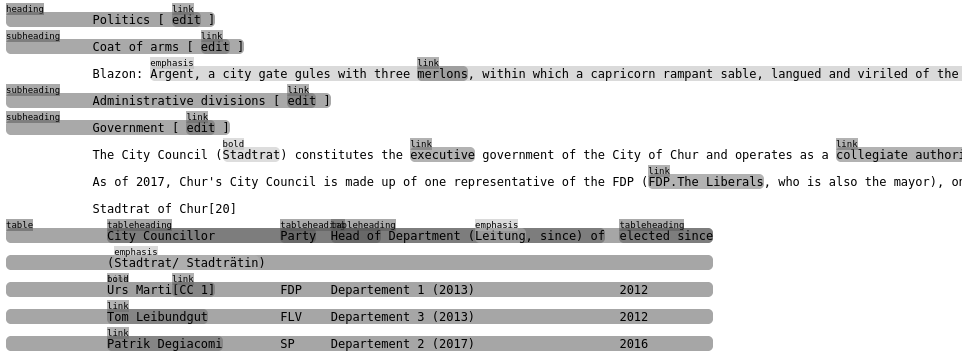
\includegraphics[width=6.3in]{inscriptis-html-postprocessor.png}
  \caption{Inscriptis - Postprocesamiento html}
  \label{img: inscriptis - postprocesamiento html}
\end{figure}

\subsection{Beautiful Soup}
\label{subsec:beautiful soup}

\emph{Beautiful Soup} \cite{beautifulsoup} es una de las librerías de Python más comunes en el ámbito del
web scraping, diseñada para extraer datos de documentos XML y HTML. Como se muestra en la tabla
\ref{tab:emparejamientos biblioteca-analizador} y a diferencia del resto de librerías, Beautiful Soup 
permite determinar el tipo de analizador que se empleará en la extracción, lo que flexibiliza el proceso 
de navegación, búsqueda y modificación de documentos.

\subsubsection{Multiplicidad de analizadores}
\label{subsubsec:multiplicidad de analizadores}

Beautiful Soup tiene a html.parse como analizador estándar de documentos HTML, pero ya hemos dicho que 
admite varios analizadores de terceros. En la tabla \ref{tab:beautiful soup - analizadores disponibles} 
se muestran los distintos analizadores disponibles, así como un pequeño resumen de las ventajas y desventajas 
de estos.

\begin{table}[h]
  \begin{center}
  \begin{tabular}{| c | c | c | c |}
  \hline \textbf{Tipo de analizador} & \textbf{Forma de uso} & \textbf{Ventajas} & \textbf{Desventajas} \\ \hline
  html & bs(markup, "html.parser") & Notablemente rapido & Mas lento que lxml \\
  lxml html & bs(markup, "lxml") & Muy rapido & Dependencia de C \\
  lxml xml & bs(markup, "xml") & Muy rapido y soporta xml & Dependencia de C \\
  html5lib & bs(markup, "html5lib") & Analiza igual que un buscador & Muy lento \\ \hline
  \end{tabular}
  \caption{Beautiful Soup - Analizadores disponibles}
  \label{tab:beautiful soup - analizadores disponibles}
  \end{center}
\end{table}

El empleo de distintos analizadores supondrá una importancia menor si se aplica sobre documentos bien 
formados, pues la solución aportada presentará la misma estructura que el propio documento original. En 
caso contrario, el uso de diferentes analizadores creará diferentes soluciones para un mismo documento. 

Se emplea el analizador lxml sobre un documento HTML sencillo pero con erratas. Vemos como la solución 
aportada propone la inclusión de nuevas etiquetas \emph{<html>} y \emph{<body>}, sin embargo, ¿qué ha 
ocurrido con la etiqueta \emph{</p>}?.

\begin{Schunk}
  \begin{Soutput}
    > BeautifulSoup("<a></p>", "lxml")
    # <html><body><a></a></body></html>
  \end{Soutput}
\end{Schunk}

En lugar de ignorar la etiqueta \emph{</p>} como lo hace lxml, el analizador html5lib la empareja con una 
etiqueta \emph{<p>} de apertura. También añade una etiqueta <head> que el analizador lxml había obviado.

\begin{Schunk}
  \begin{Soutput}
    > BeautifulSoup("<a></p>", "html5lib")
    # <html><head></head><body><a><p></p></a></body></html>
  \end{Soutput}
\end{Schunk}

Al igual que lxml, html.parse ignora la etiqueta de cierre \emph{</p>}. Podemos observar que este analizador 
ni siquiera intenta crear un documento HTML bien formado añadiendo etiquetas \emph{<html>} o \emph{<body>}.

\begin{Schunk}
  \begin{Soutput}
    > BeautifulSoup("<a></p>", "html.parser")
    # <a></a>
  \end{Soutput}
\end{Schunk}

Como vemos diferentes analizadores crearan diferentes soluciones en caso de que el documento a analizar
no este bien formado. Por ello, si deseamos analizar múltiples documentos de los que no conocemos su origen
o estructura sería deseable especificar el tipo de analizador con el fin del obtener la solución deseada.

\subsubsection{Proceso de extracción}
\label{subsubsec:proceso de extraccion}

En cuanto al proceso de extracción que se emplea en este algoritmo es sencillo. En primer lugar, el 
documento ya sea HTML o XML se convierte al completo en caracteres Unicode. Tras ello se crea un árbol de 
objetos donde cada uno de ellos representa una etiqueta o tag del propio documento. Finalmente, un 
analizador especificado por parámetro, recorre el árbol buscando las partes del mismo que se desean.

\begin{figure}[tphb]
  \centering
  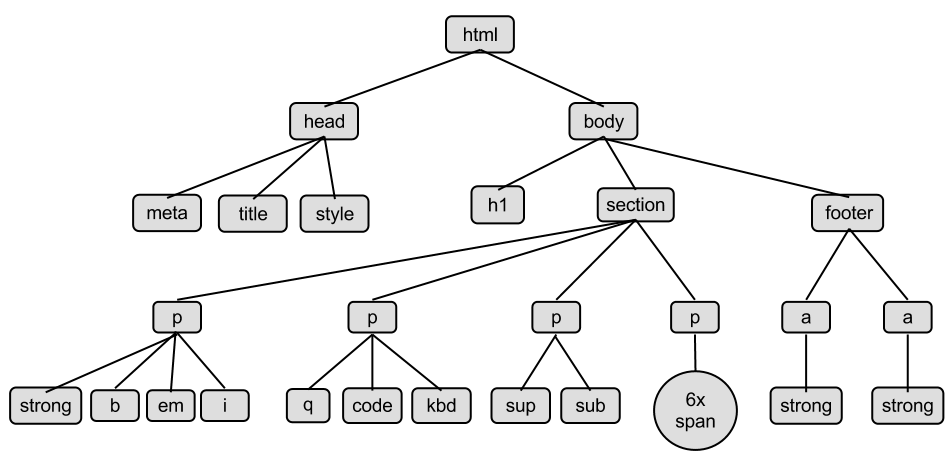
\includegraphics[width=4.5in]{bs-parse-tree.png}
  \caption{Arbol de objetos}
  \label{img:arbol de objetos}
\end{figure}

Este algoritmo, no solo permite el recorrido automático del árbol en busca del texto del documento al
completo, sino que permite además la posibilidad de recorrer el mismo de forma manual, por lo que es posible
acceder a todos los objetos del árbol empleando métodos de navegación como \emph{soup.head, soup.parent,
soup.next\_sibling, ...}.

\subsection{JusText}
\label{subsec:justext}

\emph{JusText} \cite{justext} es una herramienta para eliminar el contenido repetitivo, como los enlaces
de navegación, encabezados y pies de página de los documentos HTML. Este algoritmo, está diseñado para
preservar el texto que contiene frases completas.

\subsubsection{Preprocesamiento}
\label{subsubsec:preprocesamiento}

Previamente a cualquier fase y con el fin de facilitar el trabajo heurístico, JusText realiza un
preprocesamiento del documento HTML. Durante este proceso, se elimina el contenido de ciertas etiquetas como
\emph{<header>}, \emph{<style>} y \emph{<script>}. Además, el contenido de etiquetas como \emph{<select>}
se clasifica inmediatamente como contenido basura. Lo mismo ocurre con los bloques que contienen ciertos
símbolos especiales como el de copyright ©.

\subsubsection{Segmentación}
\label{subsubsec:segmentacion}

Tras una previa fase de preprocesamiento, se procede a lo que se conoce como segmentación. La idea es formar 
bloques de texto dividiendo la página HTML por etiquetas. Una secuencia de dos o más etiquetas como 
\emph{<br>}, \emph{<div>, ...}, separaría los bloques. 

Para la segmentación de bloques, la clave es que los bloques largos y algunos bloques cortos pueden
clasificarse con una confianza muy alta. El resto de bloques cortos pueden clasificarse observando los
bloques circundantes. 

Aunque no sea habitual, puede ocurrir que el contenido de estos bloques no sea homogéneo, es decir, que
dentro de un mismo bloque haya una mezcla de información importante con contenido basura, denominado
'boilerplate'. Se resumen a continuación algunos aspectos en relación.

\begin{itemize}
  \item Los bloques cortos que contienen un enlace son casi siempre del tipo boilerplate.
  \item Los bloques que contienen muchos enlaces son casi siempre del tipo boilerplate.
  \item Tanto los bloques buenos como los bloques de tipo boilerplate tienden a crear grupos, es decir,
  un bloque boilerplate suele estar rodeado de otros bloques de su mismo tipo y viceversa.
  \item Los bloques largos que contienen texto gramatical forman parte del contenido valioso, mientras que 
  todos los demás bloques largos son casi siempre del tipo boilerplate.
\end{itemize}

Con respecto al ultimo punto, decidir si un texto es gramatical o no puede ser complicado, JusText emplea 
una simple heurística basada en el volumen de palabras con sentido gramatical. Mientras que un texto 
gramatical suele contener un cierto porcentaje de estas palabras, los contenidos de tipo boilerplate suelen 
carecer de ellas.

\subsubsection{Clasificación de bloques}
\label{subsubsec:clasificacion de bloques}

Tras la fase de preprocesamiento y segmentación se procede a la clasificación de bloques, donde a cada uno
de estos bloques se le asigna una clase dependiendo de su naturaleza. En el fragmento de código 
\ref{cod:justext - algoritmo de clasificacion} se muestra paso a paso como se determina el tipo de clase 
para cada bloque.

\begin{codefloat}
  \inputencoding{latin1}
  \lstinputlisting[style=CppExample]{scripts/clasificacion-justext.py}
  \inputencoding{utf8}
  \caption{JusText - Algoritmo de clasificación}
  \label{cod:justext - algoritmo de clasificacion}
\end{codefloat}

Analizando el algoritmo, se observa que se definen dos tipos de variables, la densidad y la longitud. 
Mientras que la longitud es el número de caracteres por bloque, la densidad se define como la proporción 
de caracteres o palabras dentro de una etiqueta de tipo \emph{<a>}, o una lista de parada.

Además de los valores de densidad y longitud, el algoritmo toma como parámetros dos enteros definidos como
LENGTH\_LOW y LENGTH\_HIGH, y también tres números de coma flotante, MAX\_LINK\_DENSITY, STOPWORDS\_LOW y
STOPWORDS\_HIGH. Los dos primeros establecen los umbrales para dividir los bloques por su longitud. Los dos 
últimos dividen los bloques por la densidad de palabras de parada en bajos, medianos y altos.

Si volvemos a observar el algoritmo \ref{cod:justext - algoritmo de clasificacion}, nos damos cuenta de
que solo se ha realizado una clasificación real sobre los bloques de tamaño medio y largo. En la tabla
\ref{tab:justext - clasificacion de bloques long & medium size} se muestra a modo de resumen como JusText
actúa sobre este tipo de bloques.

\begin{table}[h]
  \begin{center}
  \begin{tabular}{| c | c | c |}
  \hline \textbf{Block size} & \textbf{Stopwords density} & \textbf{Class} \\ \hline
  medium size & low & bad \\ \hline
  long & low & bad \\ \hline
  medium size & medium & near-good \\ \hline
  long & medium & near-good \\ \hline
  medium size & high & near-good \\ \hline
  long & high & good \\ \hline
  \end{tabular}
  \caption{JusText - Clasificación de bloques long \& medium size}
  \label{tab:justext - clasificacion de bloques long & medium size}
  \end{center}
\end{table}

\subsubsection{Reclasificación de bloques}
\label{subsubsec:reclasificacion de bloques}

¿Qué ocurre entonces con los bloques cortos y los bloques casi buenos? La reclasificación en este caso se 
realiza en función de los bloques circundantes. Los bloques ya clasificados como buenos o malos sirven 
como piedras base en esta etapa y su clasificación se considera fiable, por lo que nunca se modifica. Esta 
reclasificación se puede ver resumida en la figura \ref{img:justext - reclasificacion de bloques}.

\begin{figure}[tphb]
  \centering
  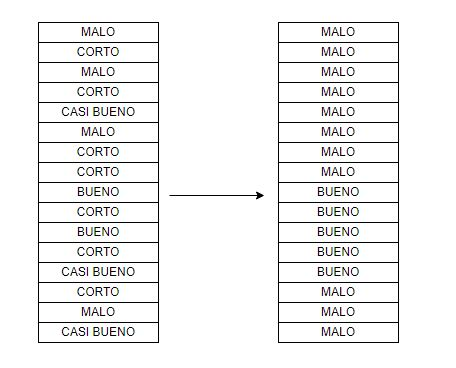
\includegraphics[width=3.6in]{justext-blocks-classification.jpg}
  \caption{JusText - Reclasificación de bloques}
  \label{img:justext - reclasificacion de bloques}
\end{figure}

La idea que subyace a la reclasificación es que los bloques boilerplate suelen estar rodeados de otros 
bloques boilerplate y viceversa. Los bloques casi buenos suelen contener datos útiles del corpus si se 
encuentran cerca de bloques buenos. Los bloques cortos suelen ser útiles sólo si están rodeados de bloques 
buenos por ambos lados.

\subsubsection{Bloques de cabecera}
\label{subsubsec:bloques de cabecera}

En cuanto a los bloques de cabecera, aquellos encerrados en etiquetas del tipo \emph{<h1>}, \emph{<h2>}, 
..., son tratados de una manera especial. El objetivo es conservar estos bloques en los textos determinados 
como buenos.

Para el tratamiento especial de bloques de cabecera se añaden dos etapas. La primera etapa, conocida como 
preprocesamiento, se ejecuta justamente después de la clasificación y justo antes de la reclasificación de 
bloques. La segunda etapa, conocida como postprocesamiento, se ejecuta después de la reclasificación.

\begin{enumerate}
  \item Clasificación de bloques.
  \item \textbf{Preprocesamiento de bloques de cabecera}.
  \item Reclasificación de bloques.
  \item \textbf{Postprocesamiento de bloques de cabecera}.
\end{enumerate}

Durante esta fase de preprocesamiento, se buscan bloques de cabecera cortos que precedan a bloques buenos, 
y que al mismo tiempo no haya más caracteres entre el bloque de cabecera y el bloque bueno. El propósito 
de esto es preservar los bloques cortos entre el encabezado y el texto bueno que, de otro modo, podrían 
ser seleccionados como malos durante el proceso de reclasificación.

Por otro lado, en el postprocesamiento, se buscan de nuevo bloques de cabecera que precedan a bloques
buenos, y que al mismo tiempo no haya más caracteres entre el bloque de cabecera y el bloque bueno. El
propósito es que algunas cabeceras cortas y casi buenas puedan clasificarse como buenas si preceden a
bloques buenos que, de otro modo, habrían sido clasificadas como malas tras de la reclasificación.

\section{Paquetes de R encontrados durante el proceso de búsqueda}
\label{sec:paquetes de r encontrados durante el proceso de busqueda}

\section{Paquetes seleccionados para el proceso de análisis}
\label{sec:paquetes seleccionados para el proceso de analisis}
